\documentclass[12pt]{article}
\usepackage[utf8]{inputenc}
\usepackage[english,french]{babel}
\usepackage{geometry}
\usepackage{graphicx}
\usepackage{fancyhdr}
\usepackage{hyperref}

%%Links
\hypersetup{
    colorlinks,
    citecolor=black,
    filecolor=black,
    linkcolor=black,
    urlcolor=black
}

\geometry{hmargin=2cm, vmargin=2cm}

\def\blurb{TDDC32 - Software Requirements Specification 1.1}

\def\ligne#1{%
  \hbox to \hsize{%
    \vbox{\centering #1}}}%

\def\abstract{%
	This document give a complete description of the behavior of the Ray Tracing Engine. This project is the main part of the TDDC32 - Design and implementation of a software module in Java course.

This document include the system descriptions, the user interface. It also include all the functional and non functional requirements for this project. At the end of this document, you can see see the use cases descriptions.

The purpose of this document is not to discuss about implementation issues but focus on how the Ray Tracing Engine will be.


}

\makeatletter
\def\maketitle{%
	\null
	\vfill
	\vbox{\centering \Large \textbf{\blurb}}
	\vspace{15mm}
	\vbox{\centering \LARGE \textbf{\@title}}
	\vspace{15mm}
	\vbox{\centering \@author}
	\vspace{8mm}
	\vbox{\centering \@date}
	\vspace{15mm}
	\vbox{\centering \textbf{Abstract}}
	\vspace{5mm}
	\vbox{%
		\setlength{\fboxsep}{10pt}
		\centering \fbox{%
		\begin{minipage}{0.9\textwidth}
			\setlength{\parindent}{1cm}
			\setlength{\parskip}{2ex plus .4ex minus .4ex}
			\abstract
		\end{minipage}%
	}
%
	}
	\vfill

}

\title{Ray Tracing Engine}
\author{Simon Vernhes \texttt{<simon@vernhes.eu>}}
\date{\today}

\begin{document}
  \pagestyle{fancyplain}
  \setlength{\parskip}{.6ex plus .4ex minus .4ex}
  \renewcommand{\headrulewidth}{0pt}
  \renewcommand{\footrulewidth}{0.6pt}
  \fancyhf{}
  \fancyhead{} 
  \lfoot{\blurb}
  \rfoot{Page \thepage}
  \maketitle \clearpage
  \tableofcontents \clearpage
  
  %\setlength{\parskip}{1ex plus .4ex minus .4ex}
  \section{Introduction}
Early, computer graphic got the ambition the produce photo realistic images.

Ray tracing is a way to produce visual images. The main advantage of this technique among others is the photorealism of produced image.

To produce an image, a ray tracing engine trace the reverse path of the light, from the virtual eye (camera) through a virtual screen (the image) and calculate the color of visible objects. You can see an example on the figure \ref{img_intro}.

\begin{figure}[ht]
  \centering
  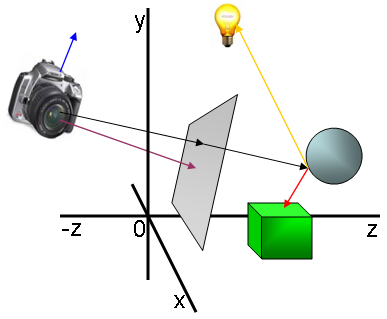
\includegraphics[height=7cm]{img/intro.png}
  \caption{Ray tracing}
  \label{img_intro}
\end{figure}

The eye (camera) look at a direction (purple arrow). A ray is traced through each pixel of the image (black arrow). The engine will try to find out where the ray intersect with an object (the sphere). The engine will find the color for this intersection by looking for the light and eventually reflexion of other objects (the cube).


  \clearpage
  \section{Document conventions}

\begin{figure}[ht]
  \centering
  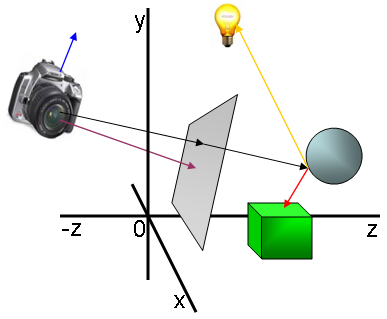
\includegraphics[height=7cm]{img/intro.png}
  \caption{Ray tracing}
\end{figure}

\begin{itemize}
  \item eye : camera
  \item viewport : plan where the eye is looking at
  \item shading effect : way to render/color a pixel (ray intersection with an object)
  \item scene : the scene the ray tracer have to render (described in the xml scene file)
\end{itemize}

  \clearpage
  \section{System description}
The ray tracing engine will be divided into 3 parts :
\begin{itemize}
  \item XML parser
  \item World objects
  \item Engine
\end{itemize}

The xml parser have an xml file as input. This xml must describe the scene which will be rendered. The syntax for this xml will be describe in the analysis phase and will be handed with a XML Scheme descriptor. This parser will produce the World object.

The world objects are all the object which can be used to describe a scene. The exhaustive list of these objects are :
\begin{itemize}
  \item Sphere
  \item Cube
  \item Cylinder
\end{itemize}

We can also do transformations on these objects : rotation, translation, scaling.

Finally, the engine will render an image using the world objects.

\begin{figure}[ht]
  \centering
  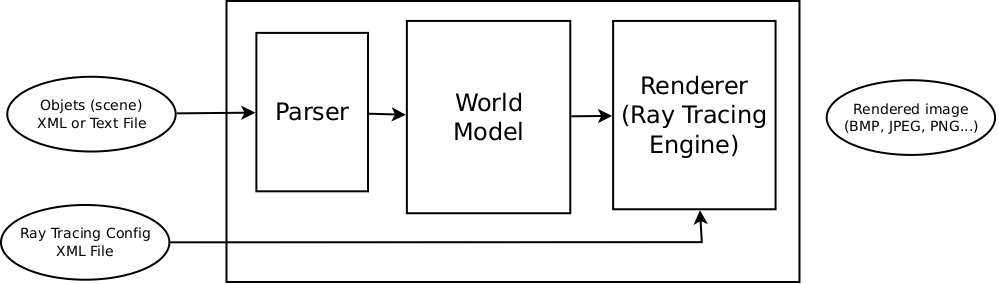
\includegraphics[height=5cm]{img/modules.png}
  \caption{Modules}
  \label{modules}
\end{figure}


  \clearpage
  \section{User interface}
The first user interface will only be command line.

The user will give a xml file as argument of the command call. Eventually a configuration for the ray tracing engine could be given. If no configuration file is given, the software will check if a file called .raytracer.xml exists in the home directory of the user (ie. $\widetilde{}/.raytracer.xml$). If not, the default parameters will be used.

Standard call :

  \texttt{\$\ raytracer -s scene.xml}

Diffenrent outputs will be provided by the program. The image must be printed on screen and also writted in a file.


  \section{System Functions}

  \subsection{Mandatory functionalities}
We expect than the ray tracing engine should be able to render basic scene, composed by sphere, cube, cylinder, plan. The will be only light, supposed to be placed at the infinite. Each object should have a color.

So, the ray tracing engine should render a single image with on input scene description xml file.

The ray tracing engine muse let the user adjust :
\begin{itemize}
  \item list of objects (sphere, cube, cylinder)
  \item parameters of these objects (position, size, rotation, color)
  \item a phong coefficient for each object
  \item a specular and diffuse reflexion for each object
  \item give the color of a unique ambient light
  \item give the position and direction of the eye
\end{itemize}

The parser should show errors in incorrect scene xml files.

  \subsection{Optional functionalities}
As optional functional, we have a lot of options.
\begin{itemize}
  \item Adding new objects : torus, more generic surface of revolution...
  \item Allowing more than one light not necessarily placed at the infinite.
  \item Adding textures to objects
  \item multi-threaded ray tracing (and eventually distrubuted among a set of machine)
  \item adding a GUI
  \item provide live view generation of the image
\end{itemize}


  \section{Non functional requirements}
No performance or security requirement for this project.

The xml scene description must be easy to create.

The software must be really sustainable.


  \section{Storage of permanent date}
Eventually, a config file could be store by the user in his home directory (i.e. $\widetilde{}/.raytracer.xml$)


  \section{Limitations}
This ray tracer is not a real-time raytracer so it firstly can only be use only to produce one image.

We will not take care of too long computations to render an image.

  \clearpage
  \section{Use Case Description}
  \subsection{General view}
The user should call the ray tracer engine providing a scene xml file. The parser will create the world objects. And finally the engine will render the image using the world objects.

\begin{figure}[ht]
  \centering
  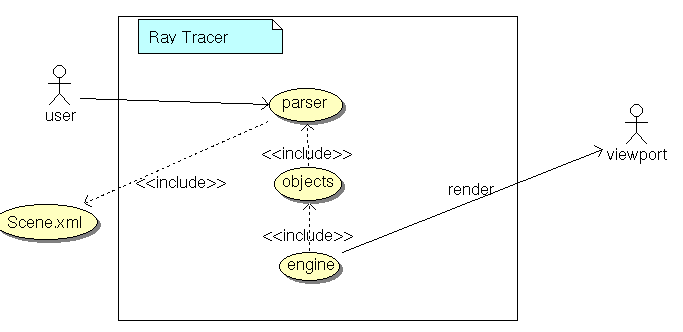
\includegraphics[height=9cm]{img/uc_raytracer.png}
  \caption{Use case general view}
  \label{img_uc_rt}
\end{figure}

  \clearpage
  \subsection{Objects}

The parser create all objects of the scene.

The creation of the camera also create the viewport.

\begin{figure}[ht]
  \centering
  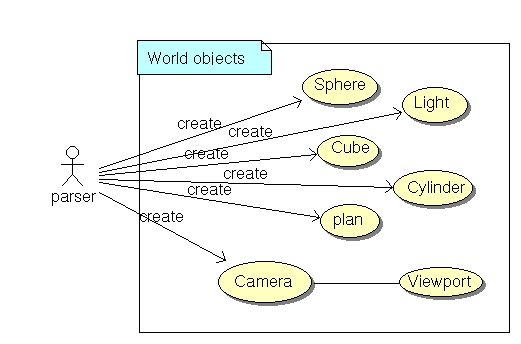
\includegraphics[height=9cm]{img/uc_objects.png}
  \caption{Use case objects creation}
  \label{img_uc_obj}
\end{figure}

  \clearpage
  \subsection{Engine}

Engine algorithm : for each pixel of the viewport, throw a ray and calculate the color where the ray intersect with an object.

\begin{figure}[ht]
  \centering
  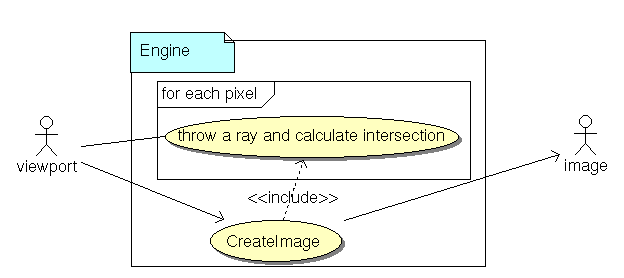
\includegraphics[height=7cm]{img/uc_render.png}
  \caption{Use case engine}
  \label{img_uc_engine}
\end{figure}




\end{document}

